% !TEX root = ./main.tex

\chapter{实验设计与结果分析}

实验验证的目标是检验平台能否真实运行、各类能力能否协同工作，以及当前方案的优势与不足。本章不追求把所有页面逐项罗列，而是围绕三类重点展开：图像虚假检测的可复验基线、图像/视频安全审核的功能链路，以及生成结果回检所形成的平台闭环。

\section{实验目标与取舍原则}

本章实验主要服务于三个目的：验证图像与视频检测链路能否从输入走到结果展示；分析本地模型与外部接口在不同任务中的适用差异；评估平台在研究验证和演示场景下的可用性。由于当前平台更强调闭环实现与方法接入，本文不做大规模跨数据集排行榜式对比，而优先保留图像检测基线、图像/视频审核链路验证、同步/异步响应分析三类内容。

需要说明的是，平台生成样本主要用于开放场景观察和生成结果回检，不直接与ProGAN定量评测样本混合计算准确率。这样处理可以避免不同来源、不同标注标准的样本被混在同一指标中，从而导致实验结论失真。

\section{实验环境与评价指标}

\subsection{实验环境}

实验在校内实验室服务器环境下完成，平台采用前后端分离与模型服务独立运行的部署方式。前端静态页面提供统一入口，后端代理服务负责请求转发、鉴权和结果归一化，本地模型服务分别承担图像虚假检测、本地文生图和本地文生视频等推理任务。

软件栈方面，前端基于React、TypeScript、Vite和Ant Design，后端基于Node.js与Express，本地推理服务基于Python、FastAPI与PyTorch。外部能力主要来自图像/视频理解接口、生成接口和视觉智能类服务。本文实验不评估硬件极限吞吐，而关注功能链路、结果结构和多源能力适配情况。

\subsection{评价指标}

图像虚假内容检测采用准确率、精确率、召回率和F1值作为主要评价指标：

\begin{equation}
Accuracy = \frac{TP + TN}{TP + TN + FP + FN}
\end{equation}

\begin{equation}
Precision = \frac{TP}{TP + FP}
\end{equation}

\begin{equation}
Recall = \frac{TP}{TP + FN}
\end{equation}

\begin{equation}
F1 = \frac{2 \times Precision \times Recall}{Precision + Recall}
\end{equation}

其中，$TP$、$TN$、$FP$、$FN$ 分别表示伪造样本正确识别、真实样本正确识别、真实样本误判为伪造和伪造样本误判为真实的数量。视频检测与安全审核当前以链路完整性、结构化返回和风险展示稳定性为主要评价角度，避免在标注数据不足时给出不可靠数值。

\section{数据集与测试样本构建}

\subsection{图像真假检测样本}

图像真假检测采用两类样本。第一类是仓库中整理完成的ProGAN测试样本，包含真实图像200张、伪造图像200张，标签明确，适合验证本地检测链路。第二类是平台生成与展示样例，包括文生图结果、人脸编辑结果和若干示例图片，用于观察开放场景表现。

实际评测中，本文从ProGAN测试集中按真实与伪造各取100张，构成平衡的 \texttt{progan\_mini} 子集，用于验证UniversalFakeDetect在当前部署环境中的推理链路。该子集不是覆盖所有生成模型，而是作为快速回归验证集，便于反复确认模型服务、后端代理和前端页面是否正常。

\begin{table}[H]
\centering
\caption{当前阶段图像真假检测样本构成}
\renewcommand{\arraystretch}{1.35}
\begin{tabular}{|C{5.0cm}|C{5.0cm}|C{2.4cm}|}
\hline
\textbf{样本来源} & \textbf{类别} & \textbf{数量} \\
\hline
ProGAN测试集 & 真实图像 & 200 \\
\hline
ProGAN测试集 & 伪造图像 & 200 \\
\hline
平台样例与生成结果 & 开放场景补充样本 & 若干 \\
\hline
\end{tabular}
\end{table}

\subsection{生成样本与安全审核样本}

生成样本主要来自平台内文生图、文生视频、图生视频、人脸替换和属性编辑等功能。它们的作用不是替代公开数据集，而是用于验证“生成—检测—审核—展示”闭环是否可运行，并观察开放场景下模型解释是否合理。对于这类样本，本文更关注输入输出链路、风险标签和人工可读说明，不使用少量生成样例推导总体准确率。

安全审核样本采用“代表性样例 + 功能链路验证”。仓库中的自然场景图像、风险场景图像、短视频样例和生成/伪造素材可覆盖安全图像、风险图像、普通视频和疑似生成视频等输入类型。平台生成结果也可作为补充样本，体现生成内容进入检测与审核模块后的闭环验证能力。

\section{图像检测与审核实验分析}

\subsection{图像虚假检测基线验证}

图像虚假检测实验验证两个问题：本地模型能否在结构化样本上稳定判断，外部多模态接口能否补充开放场景解释能力。实验分为本地模型基线验证和开放场景样例分析两部分，前者使用ProGAN样本，后者使用平台生成图片和典型示例图片。

本地图像虚假检测模块在 \texttt{progan\_mini} 子集上的阶段性结果如表~\ref{tab:ufd-progan-mini-result} 所示。结果文件由 \texttt{results\_mini/acc0.txt} 和 \texttt{results\_mini/ap.txt} 保存，其中 \texttt{acc0} 表示以0.5为阈值时的真实类准确率、伪造类准确率和总体准确率，AP表示平均精度。

\begin{table}[H]
\centering
\caption{UniversalFakeDetect在ProGAN mini子集上的链路回归结果}
\label{tab:ufd-progan-mini-result}
\small
\setlength{\tabcolsep}{2.5pt}
\renewcommand{\arraystretch}{1.35}
\begin{tabular}{|C{2.5cm}|C{1.4cm}|C{1.4cm}|C{2.25cm}|C{2.25cm}|C{2.25cm}|C{1.4cm}|}
\hline
\textbf{评测集} & \textbf{真实样本} & \textbf{伪造样本} & \textbf{真实类准确率} & \textbf{伪造类准确率} & \textbf{总体准确率} & \textbf{AP} \\
\hline
\texttt{progan\_mini} & 100 & 100 & 100.00\% & 100.00\% & 100.00\% & 100.00\% \\
\hline
\end{tabular}
\end{table}

表~\ref{tab:ufd-progan-mini-result} 的100\%结果只说明当前本地模型、后端代理和前端展示链路在小规模ProGAN同分布子集上能够稳定工作，不能直接解释为模型对所有AIGC图像都具有100\%识别率。其价值在于提供可复验的回归基线，后续仍需扩展到扩散模型样本、压缩扰动样本和真实开放场景样本。

图~\ref{fig:fake-detect-result-case} 展示了平台图像检测结果页面。该案例重点验证“上传输入—调用检测后端—解析返回—可视化展示”的完整链路。

\begin{figure}[H]
\centering
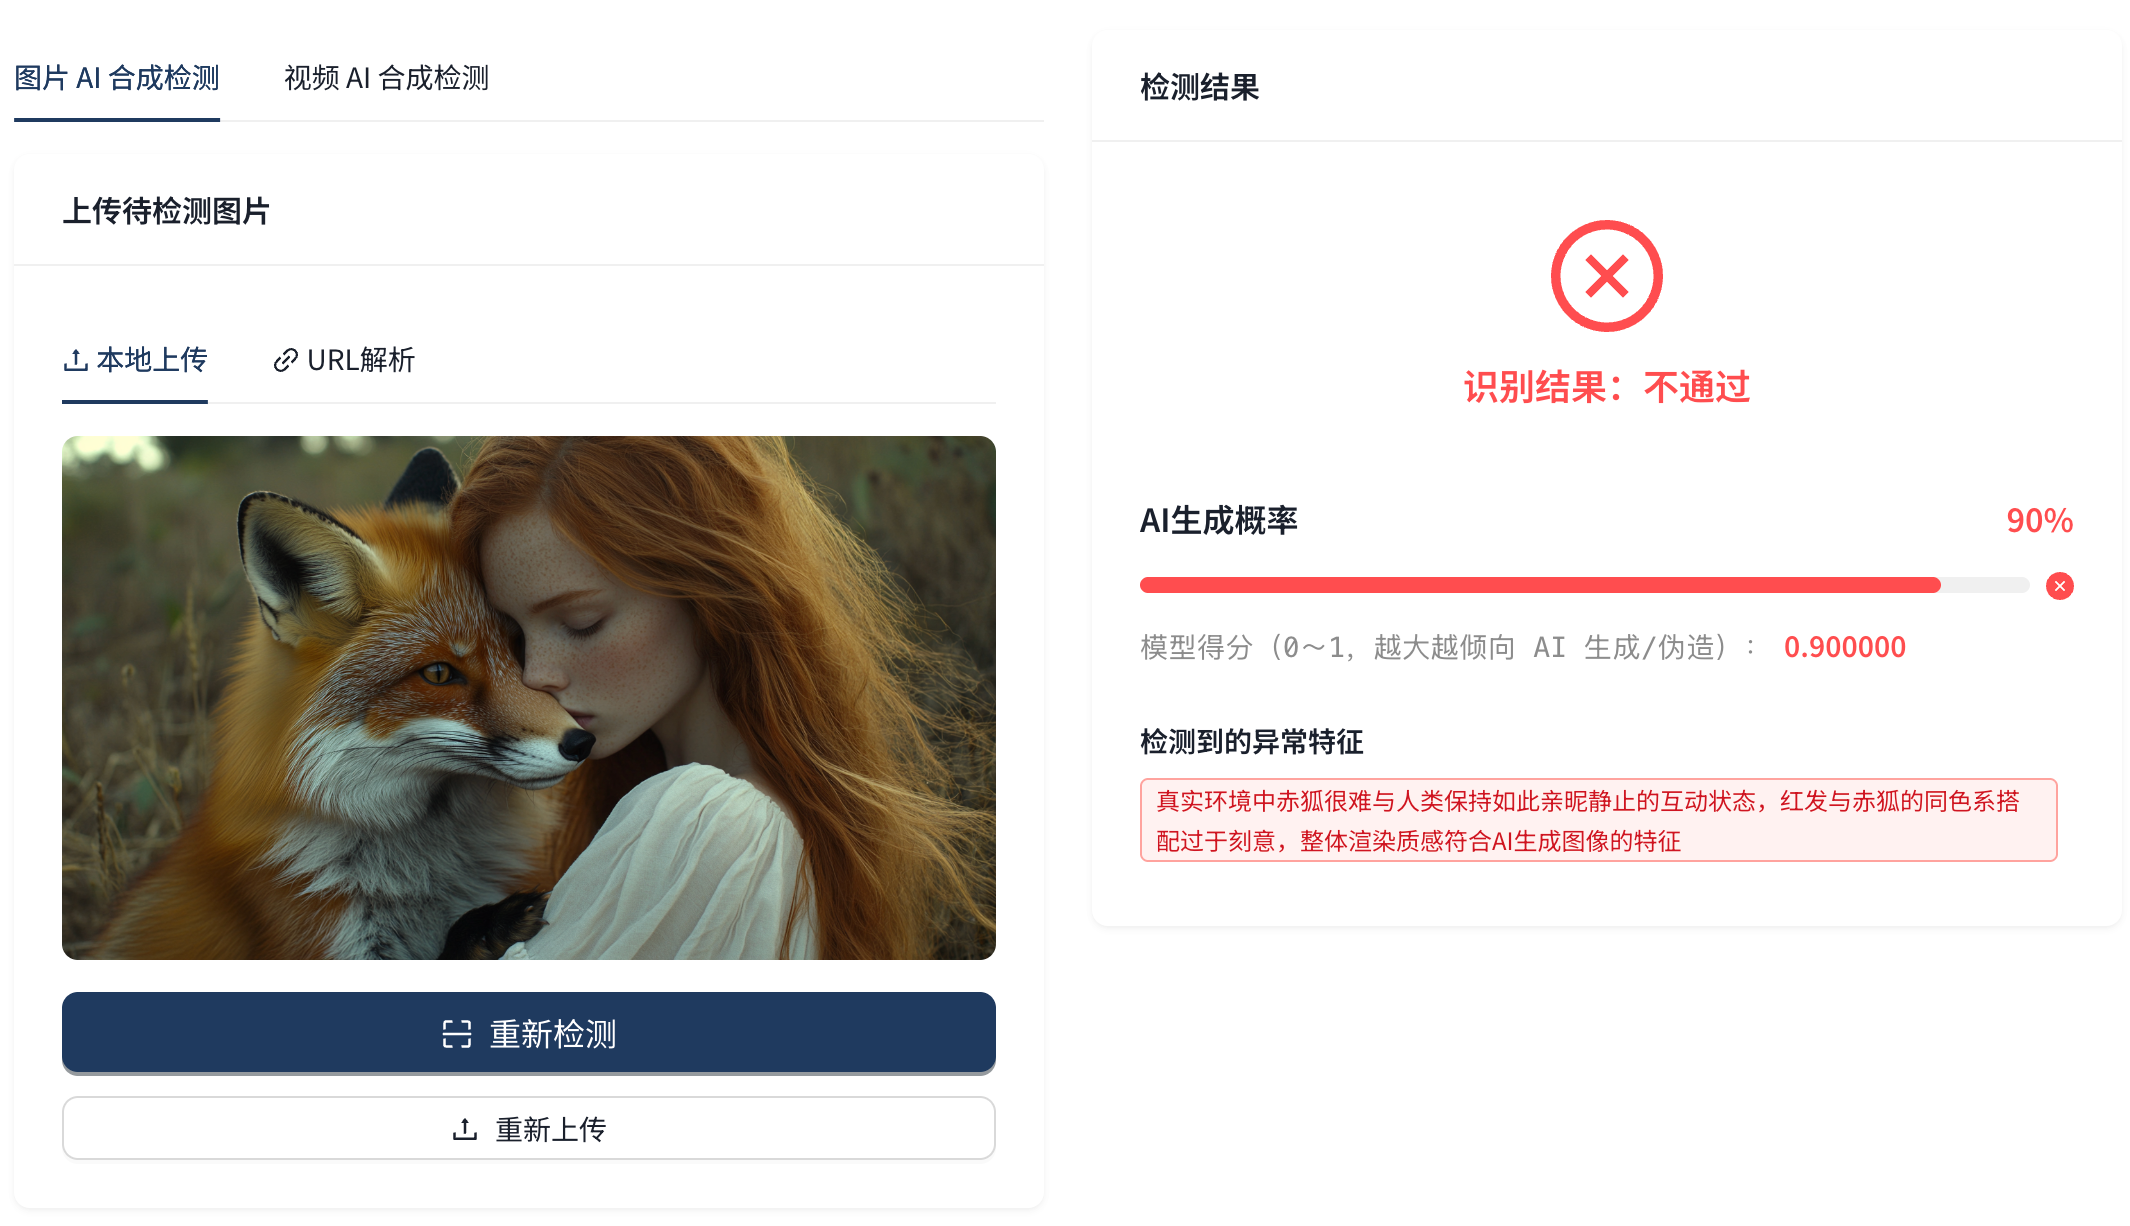
\includegraphics[width=0.98\textwidth]{figures/site-check/fake-detect-result-white.png}
\caption{图像虚假内容检测结果展示}
\label{fig:fake-detect-result-case}
\end{figure}

\subsection{图像安全审核验证}

为使图像实验同时覆盖真实性风险和内容合规风险，本文在图像虚假检测之外补充安全审核验证。图像安全审核不以真假为目标，而是验证平台能否识别风险标签、给出处置建议并把结果映射为低、中、高风险等级。该验证与图像虚假检测并列，分别覆盖真实性风险和内容合规风险。

\begin{table}[H]
\centering
\caption{图像安全审核功能验证内容}
\label{tab:image-safety-validation}
\small
\setlength{\tabcolsep}{4pt}
\renewcommand{\arraystretch}{1.35}
\begin{tabular}{|C{2.2cm}|L{3.1cm}|L{3.7cm}|L{3.6cm}|}
\hline
\textbf{验证对象} &
\multicolumn{1}{C{3.1cm}|}{\textbf{输入样本}} &
\multicolumn{1}{C{3.7cm}|}{\textbf{返回字段}} &
\multicolumn{1}{C{3.6cm}|}{\textbf{验证重点}} \\
\hline
安全图像 & 自然场景或普通人物图像 & 安全状态、建议通过、空风险标签或低风险说明 & 验证正常内容不会被误展示为高风险。 \\
\hline
风险图像 & 暴力、色情或敏感场景样例 & 风险标签、复审或阻断建议、原因说明 & 验证审核接口能输出可解释风险结果。 \\
\hline
生成图像 & 文生图或属性编辑结果 & 安全状态、风险标签、处置建议 & 验证平台生成内容可以回流到审核链路。 \\
\hline
\end{tabular}
\end{table}

图~\ref{fig:image-safety-case-placeholder} 预留图像安全审核结果截图位置，建议后续替换为一张低风险样本或一张需要复审的风险样本截图，并保证截图与说明文字出现在同一页。

\begin{figure}[H]
\centering
\screenshotplaceholder{图像安全审核结果截图占位：展示风险等级、风险标签、处置建议和原因说明}
\caption{图像安全审核结果展示占位}
\label{fig:image-safety-case-placeholder}
\end{figure}

\section{视频检测与安全审核验证}

\subsection{视频真假检测验证}

视频真假检测重点验证视频输入、统一转发、结构化返回和前端展示链路。当前平台主要通过多模态视频理解接口实现，支持视频链接或本地短视频输入，并返回真假结论、置信度和文本说明。当前实现还支持抽帧频率参数，用于在视频理解任务中控制采样密度。

\subsection{视频安全审核验证}

视频安全审核重点验证整段视频内容能否进入安全审核链路，并返回安全状态、风险标签、处置建议和原因说明。与图像审核相比，视频审核更关注动作过程和时序语义，因此当前阶段以链路完整性和结构化结果为主要评价对象，不给出大规模准确率。

\subsection{功能验证结果讨论}

视频与安全审核的代表性验证内容如表~\ref{tab:video-safety-validation} 所示。表中未给出大规模准确率，是因为当前样本尚未形成严格标注数据集；本文更关注稳定输入、结构化返回和统一展示能力，并为后续定量实验保留接口基础。

\begin{table}[H]
\centering
\caption{视频检测与安全审核功能验证内容}
\label{tab:video-safety-validation}
\small
\setlength{\tabcolsep}{4pt}
\renewcommand{\arraystretch}{1.35}
\begin{tabular}{|C{2.5cm}|L{3.0cm}|L{4.3cm}|L{4.2cm}|}
\hline
\textbf{验证任务} &
\multicolumn{1}{C{3.0cm}|}{\textbf{输入形式}} &
\multicolumn{1}{C{4.3cm}|}{\textbf{返回字段}} &
\multicolumn{1}{C{4.2cm}|}{\textbf{验证重点}} \\
\hline
视频AI生成检测 & 视频URL或本地短视频Base64 & 真假结论、置信度、模型名称、原因说明 & 验证视频输入能否通过后端统一转发并映射为虚假检测结果。 \\
\hline
视频安全审核 & 视频URL或本地短视频Base64 & 安全状态、风险标签、处置建议、原因说明 & 验证视频审核链路能否与图像审核共享展示逻辑。 \\
\hline
生成结果回检 & 平台生成图片或视频 & 真假检测结果或安全审核结果 & 验证“生成—检测—展示”闭环是否可运行。 \\
\hline
\end{tabular}
\end{table}

图~\ref{fig:video-validation-placeholder} 预留视频检测或视频安全审核截图位置。该截图应优先展示视频预览、fps参数、检测结论和原因说明，从而体现当前视频链路的关键实现点。

\begin{figure}[H]
\centering
\screenshotplaceholder{视频检测或视频安全审核截图占位：展示视频预览、fps参数、检测结论、风险标签和说明文本}
\caption{视频检测与审核结果展示占位}
\label{fig:video-validation-placeholder}
\end{figure}

\section{系统响应特征与可用性分析}

\subsection{响应特征分析}

平台按任务耗时组织响应模式。图像检测和图像审核属于轻量同步任务，适合直接返回；视频生成、图生视频和部分视频理解任务属于长链路任务，需要后端轮询和状态封装。不同任务的响应方式如表~\ref{tab:response-mode} 所示，这也是后端代理层存在的直接原因之一。

\begin{table}[H]
\centering
\caption{不同任务的响应组织方式}
\label{tab:response-mode}
\small
\setlength{\tabcolsep}{4pt}
\renewcommand{\arraystretch}{1.35}
\begin{tabular}{|C{2.5cm}|C{2.0cm}|L{4.5cm}|L{4.4cm}|}
\hline
\textbf{任务类型} &
\textbf{响应模式} &
\multicolumn{1}{C{4.5cm}|}{\textbf{后端处理重点}} &
\multicolumn{1}{C{4.4cm}|}{\textbf{前端展示重点}} \\
\hline
图像虚假检测 & 同步返回 & Base64或URL转发、分数与字段归一化 & 显示真假标签、置信度和模型说明。 \\
\hline
图像安全审核 & 同步返回 & 审核JSON提取、标签与建议映射 & 显示风险等级、风险标签和处理建议。 \\
\hline
视频检测与审核 & 同步或较长请求 & 视频URL/Base64封装、fps参数、结构化结果解析 & 显示视频预览、置信度和说明文本。 \\
\hline
文生视频/图生视频 & 异步轮询 & 任务提交、状态查询、超时控制和结果URL提取 & 显示加载状态、生成结果和失败提示。 \\
\hline
\end{tabular}
\end{table}

\subsection{平台可用性分析}

平台可用性取决于交互链路是否清晰。当前系统已形成内容输入、任务选择、结果展示和样本回流的基本闭环，覆盖首页导航、内容生成、真假检测、安全审核和结果查看等流程。后端代理层屏蔽多源接口差异，并通过错误提示和结构化返回降低理解成本。

从实验使用角度看，当前平台已经能够支撑毕业设计阶段的功能验证：图像真假检测具备可复验本地基线，图像和视频安全审核具备统一风险展示，通用生成与Deepfake生成可以为检测模块提供开放场景样本。其不足主要在于视频本地检测模型尚未补强、数据管理仍以页面展示为主、生成样本规模不足以支撑严格统计结论。

\section{实验结果综合分析}

综合实验可知，平台已在图像检测、视频检测和不安全内容审核三个方向形成业务链路。图像任务最成熟，本地模型与外部接口的双后端方案为后续量化对比奠定基础；视频与安全审核目前偏功能验证，但接入方式稳定，为扩展本地视频模型和大规模审核实验保留了入口。生成模块的价值主要体现在样本构建和闭环演示，而不是直接作为定量评测集。

\section{本章小结}

本章根据当前项目进展，明确了实验取舍原则，将图像虚假检测作为可复验基线，将图像/视频安全审核作为功能链路验证方向，并从响应特征和交互流程分析平台可用性。结果表明，平台已完成从内容生成、内容检测到风险展示的基本闭环，但在视频本地检测、样本规模和大规模定量评估方面仍有提升空间。
